\section{Обзор литературы}
\subsection{Система декларативного управления кластером \textit{GitOps}}
\label{sec:gitops}
\textit{GitOps} -- это подход к автоматизации и управлению инфраструктурой, в котором используется система контроля версий \textit{Git} как единственный источник истины для всей инфраструктуры и приложений. Этот метод активно используется для управления \textit{Kubernetes}-кластерами и другими контейнеризованными приложениями. В отличие от традиционных методов управления инфраструктурой, где операции выполняются вручную или с помощью инструментов, таких как \textit{Ansible} или \textit{Terraform}, в \textit{GitOps} все изменения конфигурации управляются через \textit{Git}. 

\subsubsection{История и развитие \textit{GitOps}.}
Подход \textit{GitOps} был предложен в 2017 году компанией \textit{Weaveworks} и быстро получил признание среди разработчиков, работающих с \textit{Kubernetes}. Идея заключалась в том, чтобы использовать один инструмент -- \textit{Git} -- для всего цикла жизни инфраструктуры. Это позволило упростить процессы управления конфигурациями и повысить безопасность, поскольку все изменения теперь могли быть отслежены и автоматически применены через \textit{CI/CD} пайплайны.

\subsubsection{Применение \textit{GitOps}\ref{gitops}.}
Этот подход применим в средах, где используется контейнеризация и микросервисная архитектура. Он используется для автоматического применения изменений в инфраструктуре на основе изменений в репозиториях \textit{Git}, что позволяет упростить развертывание новых версий приложений и настройку инфраструктуры. В случае с \textit{Kubernetes} это обеспечивает централизованное и повторяемое управление конфигурациями кластеров и приложений, гарантируя согласованность между желаемым состоянием в \textit{Git} и реальным состоянием в кластере. Это дает преимущества в плане управления версиями, аудитирования и восстановления состояния, что особенно важно для крупных и динамичных систем.

\subsubsection{Выбор инструмента для реализации \textit{GitOps: FluxCD vs ArgoCD}.}
Для реализации подхода \textit{GitOps} существует несколько популярных инструментов, среди которых наиболее известными являются \textit{FluxCD} и \textit{ArgoCD}. Оба инструмента предлагают решения для автоматического применения конфигураций, хранящихся в \textit{Git}, и позволяют интегрировать процессы развертывания и мониторинга изменений. Однако каждый из них имеет свои особенности, преимущества и недостатки.


\textit{ArgoCD}\ref{gitops} -- это мощный и гибкий инструмент для управления развертываниями в \textit{Kubernetes}, который поддерживает декларативный подход и интеграцию с \textit{Git}. Он имеет множество функций, включая:

\begin{itemize}
    \item поддержка нескольких репозиториев \textit{Git}, что позволяет управлять несколькими проектами или кластерами; 
    \item визуальный интерфейс, позволяющий легко отслеживать состояние развернутых приложений и просматривать историю изменений; 
    \item поддержка различных стратегий развертывания, таких как \textit{Blue-Green Deployment} и \textit{Canary Releases}; 
    \item интеграция с инструментами мониторинга и уведомлений, что позволяет оперативно реагировать на проблемы. 
\end{itemize}

Однако \textit{ArgoCD} может быть более сложным в настройке, особенно для небольших проектов, и требует дополнительных усилий для интеграции с другими системами. Его визуальный интерфейс также может быть избыточным для некоторых пользователей, предпочитающих работать исключительно с командной строкой.


\textit{FluxCD} -- это более легковесный и простой инструмент~\cite{fluxcd}, ориентированный на декларативное управление инфраструктурой через \textit{Git}. Он интегрируется с \textit{Kubernetes} и автоматически синхронизирует состояние кластера с конфигурациями, хранящимися в репозитории. Ключевые особенности \textit{FluxCD} включают:

\begin{itemize}
    \item простота в настройке и интеграции, что делает его удобным для использования в небольших и средних проектах; 
    \item поддержка \textit{GitOps} на базе \textit{GitHub}, \textit{GitLab} и других сервисов, а также возможность работы с несколькими репозиториями; 
    \item высокая степень автоматизации, включая автоматическое обновление приложений при изменении конфигураций в \textit{Git}; 
    \item меньшая нагрузка на систему, благодаря минималистичному подходу и отсутствию дополнительного пользовательского интерфейса. 
\end{itemize}

Одним из недостатков \textit{FluxCD} является его ограниченная поддержка некоторых продвинутых функций, таких как стратегии развертывания (\textit{Blue-Green Deployment} или \textit{Canary Releases}), которые присутствуют в \textit{ArgoCD}. Однако, для большинства сценариев, связанных с \textit{GitOps}, этого достаточно.

В процессе выбора инструмента для реализации \textit{GitOps} была проведена оценка нескольких факторов, включая сложность настройки, масштабируемость, поддержку и требования к функционалу. Для решения задач, связанных с автоматизацией развертывания и управления \textit{Kubernetes}-кластерами в рамках корпоративной инфраструктуры, был выбран \textit{FluxCD} по следующим причинам:

\begin{enumerate}
    \item Более чистый \textit{GitOps}-like подход -- в отличие от \textit{ArgoCD}, \textit{FluxCD} использует чисто декларативный подход с полной интеграцией \textit{Git}, используя \textit{Custom Resource Definitions (CRD)} для управления состоянием кластера, что обеспечивает более правильный и стабильный механизм работы с \textit{Kubernetes} и его ресурсами.
    \item Отсутствие совмещения декларативного и императивного подходов \textit{FluxCD} фокусируется исключительно на декларативном управлении, что позволяет устранить возможные сложности, связанные с совмещением императивных и декларативных подходов в одном инструменте.
    \item Простота в использовании и настройке -- \textit{FluxCD} имеет низкий порог входа и позволяет быстро интегрировать его в существующие \textit{Kubernetes} кластеры без необходимости использования дополнительных сложных интерфейсов.
    \item Легковесность -- \textit{FluxCD} обладает минималистичной архитектурой, что подходит для среды, где важна производительность и где не требуется избыточный функциональность.
    \item Высокая степень автоматизации -- \textit{FluxCD} автоматически синхронизирует состояние кластера с конфигурациями в \textit{Git}, что упрощает процесс управления инфраструктурой и устраняет необходимость вручную поддерживать состояние.
    \item Поддержка \textit{GitOps} для нескольких репозиториев -- \textit{FluxCD} легко интегрируется с различными репозиториями, что позволяет организовать централизованное управление несколькими приложениями и сервисами.
    \item Хорошая поддержка сообществом и документацией -- \textit{FluxCD} имеет активное сообщество и исчерпывающую документацию, что обеспечивает легкость в решении проблем и внедрении новых функциональных возможностей. 
\end{enumerate}

В итоге, несмотря на то, что \textit{ArgoCD} имеет более развитые возможности визуализации и развертывания, для данной инфраструктуры, ориентированной на простоту, автоматизацию и легкость в использовании, \textit{FluxCD} оказался более подходящим инструментом благодаря своему более чистому подходу и глубокой интеграции с \textit{Kubernetes}.

\subsection{Система контроля версий \textit{Git}}
\label{sec:git}
\textit{Git}\ref{git} -- это распределенная система контроля версий, изначально разработанная Линусом Торвальдсом в 2005 году для поддержки разработки ядра операционной системы \textit{Linux}. \textit{Git} позволяет разработчикам отслеживать изменения в коде, работать над проектами в команде, и объединять изменения в единое целое.

\subsubsection{Особенности и принципы работы \textit{Git}.}
Одной из основных особенностей \textit{Git} является его распределенная природа. В отличие от централизованных систем контроля версий, таких как \textit{Subversion}, где существует один центральный репозиторий, \textit{Git} позволяет каждому пользователю хранить локальную копию репозитория. Это ускоряет процессы работы с кодом, повышает безопасность и делает систему более устойчивой к сбоям.

\subsubsection{Git в контексте управления инфраструктурой.}
\textit{Git} активно используется в подходе \textit{GitOps}, как основной инструмент для автоматизации развертывания инфраструктуры и приложений. Все изменения, касающиеся настройки инфраструктуры или конфигурации приложений, коммитятся в репозиторий \textit{Git}, откуда автоматически распространяются на рабочие системы, через инструменты \textit{CI/CD}, такие как \textit{Jenkins} или \textit{GitLab CI}.

\subsection{Система оркестрации \textit{Kubernetes}}
\label{sec:kubernetes}
\textit{Kubernetes} -- это система оркестрации контейнеров с открытым исходным кодом~\cite{kubernetes}, разработанная компанией \textit{Google} и переданная в \textit{Cloud Native Computing Foundation (CNCF)} в 2014 году. \textit{Kubernetes} предоставляет средства для автоматизации развертывания, масштабирования и управления контейнеризованными приложениями в различных средах -- от локальных серверов до облачных инфраструктур.

\subsubsection{История \textit{Kubernetes}.}
Разработка \textit{Kubernetes} началась в \textit{Google} как внутренний проект, на основе системы управления контейнерами \textit{Borg}, которая использовалась для управления вычислительными ресурсами в масштабах всей компании. В 2014 году проект был выпущен как открытый исходный код, и с тех пор он стал де-факто стандартом для оркестрации контейнеров в облачных и локальных инфраструктурах.

\subsubsection{Основные компоненты \textit{Kubernetes}.} Среди них однозначно можно выделить следующий ряд компонентов:
\begin{enumerate}
    \item \textit{Pod} -- наименьшая и базовая единица развертывания в \textit{Kubernetes}, которая может содержать один или несколько контейнеров.
    \item \textit{ReplicaSet} -- гарантирует наличие нужного числа реплик \textit{Pod}-ов, что обеспечивает отказоустойчивость.
    \item \textit{Deployment} -- управляет версиями и обновлениями приложения, развернутого в контейнерах.
    \item \textit{Service} -- абстракция, которая определяет, как контейнеры могут взаимодействовать друг с другом и с внешними клиентами.
    \item \textit{Ingress} -- управляет входящими \textit{HTTP} и \textit{HTTPS} запросами в кластер.
\end{enumerate}

\subsubsection{Применение \textit{Kubernetes}.}
\textit{Kubernetes} широко используется для автоматизации развертывания и масштабирования микросервисных приложений. Он позволяет эффективно управлять большими кластерами контейнеров и обеспечивает высокую доступность и отказоустойчивость приложений. \textit{Kubernetes} является неотъемлемой частью большинства современных облачных инфраструктур и используется во многих крупных организациях.

\subsection{Система декларативного управления инфраструктрой \textit{Terraform}}
\label{sec:terraform}
\textit{Terraform} -- это инструмент для управления инфраструктурой как кодом, реализуя подход (\textit{Infrastructure as Code (IaC)}), с открытым исходным кодом, который позволяет пользователям описывать инфраструктуру с помощью декларативных конфигурационных файлов. Он был разработан компанией \textit{HashiCorp} и позволяет управлять ресурсами облачных провайдеров, такими как \textit{Amazon Web Services (AWS)}, \textit{Google Cloud}, \textit{Azure}, а также локальными ресурсами.

\subsubsection{Особенности и использование \textit{Terraform}.}
Одним из главных преимуществ \textit{Terraform}\cite{terraform} является возможность управления инфраструктурой на различных облачных платформах с использованием единого инструмента. \textit{Terraform} использует язык конфигурации \textit{HCL (HashiCorp Configuration Language)}, который прост в освоении и позволяет описывать инфраструктуру декларативным способом. Инструмент создает, изменяет и отслеживает состояние инфраструктуры, что позволяет автоматизировать процессы развертывания и управления ресурсами.
\subsection{Система декларативного управления конфигурацией \textit{Ansible}}
\label{sec:ansible}
\textit{Ansible} -- это инструмент автоматизации для управления конфигурациями, развертывания приложений и задач по оркестрации. Он был разработан компанией \textit{Red Hat} и используется для автоматизации рутинных операций и ускорения процессов развертывания.

\subsubsection{Особенности и принципы работы \textit{Ansible}.}
Одним из главных преимуществ \textit{Ansible} является его простота в использовании. Он использует простой язык \textit{YAML} для описания конфигураций и задач, что делает его доступным для администраторов и разработчиков. \textit{Ansible} не требует агентов на целевых машинах, что упрощает настройку и управление. В отличие от других инструментов автоматизации, таких как \textit{Puppet} и \textit{Chef}, \textit{Ansible} применяет императивный подход, что означает, что его конфигурации не зависят от состояния системы, а описывают последовательность действий, которые необходимо выполнить. 

\textit{Ansible} также поддерживает концепци \textit{idempotence} (идемпотентности), что позволяет многократно выполнять одни и те же задачи без риска вызвать неправильное состояние системы. Это особенно важно для обеспечения консистентности в управляемых системах.

\subsubsection{Применение \textit{Ansible}.}
\textit{Ansible} активно используется для автоматизации развертывания приложений, управления конфигурациями серверов, а также оркестрации процессов в инфраструктуре. Он идеально подходит для следующих задач:
\begin{itemize}
    \item управление конфигурациями серверов и приложений, включая установку, настройку и обновление программного обеспечения;
    \item оркестрация развертываний и процессов, включая настройку окружений для различных приложений и сервисов;
    \item обеспечение безопасности инфраструктуры с помощью автоматизации обновлений, патчей и проверки соответствия стандартам безопасности;
    \item интеграция с другими инструментами автоматизации, такими как \textit{Docker}, \textit{Kubernetes}, \textit{AWS}, для более комплексной автоматизации и оркестрации.
\end{itemize}

\subsubsection{Выбор инструмента для автоматизации управления состоянием системы}
В процессе выбора инструмента для автоматизации конфигурации и управления инфраструктурой, была проведена оценка нескольких инструментов: \textit{Ansible}, \textit{Puppet} и \textit{Chef}. Каждый из этих инструментов имеет свои особенности и преимущества, которые могут быть важны в зависимости от масштабов инфраструктуры, специфики задач и предпочтений команды.


\textit{Puppet} -- это мощный инструмент для управления конфигурациями, ориентированный на декларативный подход. Он позволяет описывать желаемое состояние системы, и автоматически вносить изменения, чтобы привести систему в это состояние. Среди особенностей \textit{Puppet}:
\begin{itemize}
    \item мощная система управления конфигурациями, которая предоставляет обширные возможности для настройки и применения политик безопасности;
    \item поддержка различных операционных систем и платформ, включая \textit{Linux} и \textit{Windows};
    \item использование собственного языка \textit{Puppet DSL}, что требует дополнительных усилий для обучения и освоения.
\end{itemize}

Стоит отметить, что \textit{Puppet} может быть сложным в настройке и требует использования агентов на целевых системах, что добавляет сложности в процессе управления. Это делает его менее подходящим для сред с высокой динамикой и малым числом серверов.


\textit{Chef} также является мощным инструментом для управления конфигурациями, ориентированным на императивный подход. Он использует \textit{Ruby}-скрипты для описания конфигураций, что позволяет создавать очень гибкие и сложные задачи. К однозначным преимуществам \textit{Chef} можно отнести:
\begin{itemize}
    \item высокий уровень гибкости и возможности для создания сложных конфигураций;
    \item использование языка \textit{Ruby}, что может быть непривычно для администраторов, не знакомых с этим языком.
\end{itemize}

\textit{Chef} требует большего времени на обучение и внедрение, особенно для небольших и средних проектов. Его подход может быть избыточным в случаях, когда необходимы простота и скорость развертывания.


\textit{Ansible}, в свою очередь, является наиболее простым в использовании и легким для внедрения инструментом из рассмотренных вариантов. Он идеально подходит для сред, где требуется быстрая и простая автоматизация без сложной настройки и использования агентов. Преимущества \textit{Ansible}:
\begin{itemize}
    \item простой и читаемый язык \textit{YAML} для описания конфигураций, что позволяет легко интегрировать его с процессами \textit{CI/CD};
    \item отсутствие необходимости в установке агентов на целевых системах, что упрощает настройку и управление;
    \item хорошая поддержка как для одноразовых задач, так и для регулярных процессов управления инфраструктурой;
    \item большая гибкость благодаря богатой экосистеме модулей и поддержке множества различных провайдеров облачных сервисов и виртуализаций.
\end{itemize}

\subsubsection{Почему был выбран \textit{Ansible}.}
В процессе выбора инструмента для автоматизации конфигурации и управления инфраструктурой был выбран \textit{Ansible} по следующим причинам:
\begin{itemize}
    \item простота в использовании и конфигурации, что позволяет быстро начать автоматизацию и не требует глубоких знаний в программировании;
    \item отсутствие необходимости в установке агентов на целевых системах, что упрощает администрирование и снижает затраты на поддержку;
    \item поддержка широкого спектра технологий и платформ, что позволяет интегрировать его с существующими системами и сервисами;
    \item высокий уровень автоматизации и возможность интеграции с другими инструментами автоматизации и оркестрации, такими как \textit{Docker}, \textit{Kubernetes}, \textit{AWS} и другими.
\end{itemize}

Таким образом, \textit{Ansible}~\cite{ansible} оказался наиболее подходящим инструментом для реализации автоматизации и управления конфигурациями в инфраструктуре, ориентированной на скорость, гибкость и простоту в настройке.

\subsection{Система мониторинга (\textit{Grafana Stack})}
\label{sec:monitoring}
Для обеспечения стабильности и высокой доступности инфраструктуры важным аспектом является мониторинг. \textit{Grafana Stack}~\cite{grafana} включает в себя \textit{Prometheus}~\cite{prometheus}, который собирает и хранит метрики, и \textit{Grafana}, которая визуализирует данные и отображает их в виде панелей мониторинга.

\subsubsection{Использование \textit{Grafana} для мониторинга.}
\textit{Grafana} позволяет создавать динамические и настраиваемые дашборды для мониторинга состояния инфраструктуры, включая показатели нагрузки на серверы, использование ресурсов, ошибки и другие метрики. 

\subsubsection{Использование \textit{Prometheus} для сбора метрик.}
\textit{Prometheus} является одним из ведудущих инструментов для сбора, хранения и аггрегации метрик. В рамках системы мониторинга, сервис обеспечивает централизоавнный сбор метрик с приложений, серверов и других компонентов инфраструктуры.

\subsection{Организация удаленного доступа к инфраструктуре}
\label{sec:vpn}
\textit{OpenVPN} -- это популярное решение для создания виртуальных частных сетей (\textit{VPN})\cite{openvpn}, которое позволяет пользователям безопасно подключаться к корпоративной сети через интернет.

\begin{figure}[ht]
    \centering
    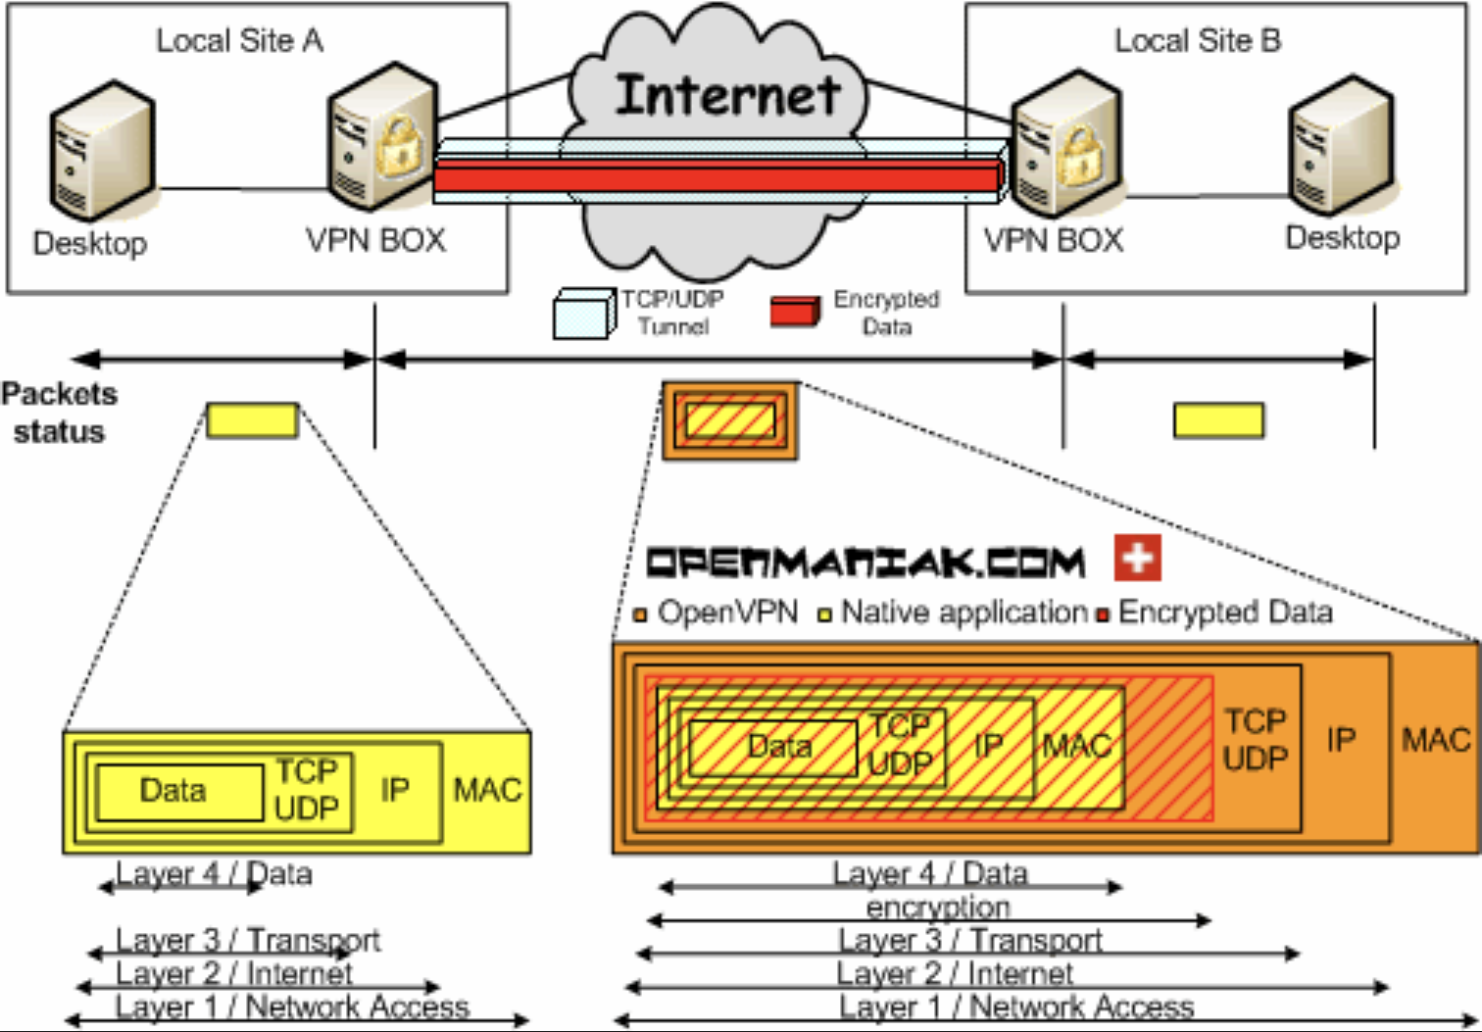
\includegraphics[width=0.7\linewidth]{\commonSecPathPrefix/../img/openvpn.png}
    \caption{Диаграмма подключений к \textit{OpenVPN}}
    \label{fig:user_guide:openvpn_diagram}
\end{figure}

\subsubsection{Как работает \textit{OpenVPN}.}
\textit{OpenVPN} использует протоколы шифрования для защиты данных, передаваемых через общественные сети. Он поддерживает различные методы аутентификации и шифрования, включая сертификаты и двухфакторную аутентификацию, что повышает безопасность подключения.

Основой работы \textit{OpenVPN} являются два режима сетевого интерфейса: \textit{TUN} и \textit{TAP}. Режим \textit{TUN} создает виртуальный IP-интерфейс уровня \textit{L3}, обеспечивая туннелирование \textit{IP}-пакетов. Он чаще всего используется для маршрутизируемых \textit{VPN}-сетей и позволяет создавать безопасные соединения на уровне сетевого слоя. Режим \textit{TAP} создает виртуальный \textit{Ethernet}-интерфейс уровня \textit{L2}, позволяя передавать не только \textit{IP}-пакеты, но и другие протоколы, что полезно для организации мостовых сетей и работы с протоколами, требующими широковещательных сообщений.

\subsubsection{Адресация и конфигурирование.}
Для организации адресации \textit{OpenVPN} может работать с различными схемами назначения \textit{IP}-адресов клиентам. Наиболее распространенным является использование внутреннего пула адресов, выделяемого сервером, из которого каждому клиенту при подключении динамически назначается уникальный \textit{IP}-адрес. Такой подход упрощает управление и предотвращает конфликты в адресации.

Кроме того, \textit{OpenVPN} поддерживает статическое назначение \textit{IP}-адресов клиентам на основе их сертификатов или уникальных идентификаторов. Это полезно для настройки постоянных маршрутов и ограничения доступа к ресурсам сети.

\textit{OpenVPN} предоставляет гибкие возможности для динамического конфигурирования клиентов. Сервер может передавать клиентам дополнительные параметры, такие как маршруты, \textit{DNS}-серверы, настройки прокси и скрипты запуска, что облегчает интеграцию \textit{VPN} в существующую инфраструктуру.

Поддержка скриптов и плагинов позволяет автоматизировать процессы аутентификации, авторизации и управления подключениями, включая взаимодействие с внешними системами управления пользователями и базами данных.

\subsubsection{Применение \textit{OpenVPN}.}
\textit{OpenVPN} используется для обеспечения безопасного удаленного доступа к корпоративной сети, что особенно важно для организаций с распределенными командами и удаленными сотрудниками. Использование \textit{OpenVPN} позволяет создать защищенный канал связи, который обеспечивает конфиденциальность и целостность передаваемых данных.

Благодаря широким возможностям настройки, \textit{OpenVPN} может быть адаптирован для различных сценариев: от простых \textit{VPN}-соединений для удаленного доступа до сложных многоуровневых архитектур с балансировкой нагрузки и высокой отказоустойчивостью.

Кроме того, \textit{OpenVPN} совместим с большинством операционных систем и устройств, включая мобильные платформы, что обеспечивает универсальность решения и удобство для конечных пользователей.

Важной особенностью \textit{OpenVPN} является поддержка различных методов аутентификации и возможности интеграции с существующими системами управления доступом, такими как \textit{LDAP} и \textit{RADIUS}. Это позволяет централизованно контролировать права пользователей и повышает уровень безопасности, снижая риски несанкционированного доступа.

Таким образом, внедрение \textit{OpenVPN} в корпоративную инфраструктуру позволяет повысить безопасность и гибкость организации удаленного доступа, обеспечивая при этом удобство управления и масштабируемость.

\subsection{Обзор существующих аналогов}
\label{sec:existing_analogs}
На современном рынке существует множество облачных платформ и инструментов для автоматизации развертывания инфраструктуры и управления ей. Среди них выделяются:
\begin{enumerate}
    \item \textit{Amazon Web Services (AWS)} -- один из крупнейших облачных провайдеров, предоставляющий широкий спектр услуг для развертывания и управления инфраструктурой.
    \item \textit{Yandex.Cloud} -- облачная платформа, предлагающая облачные сервисы для создания и управления инфраструктурой с учетом специфики российского рынка\cite{yandexcloud}.
    \item \textit{Azure} -- облачная платформа от \textit{Microsoft}, предлагающая широкий набор сервисов для бизнеса.
    \item \textit{Google Cloud Platform (GCP)} -- облачная платформа от компании \textit{Google}, которая предоставляет инструменты для развертывания и управления приложениями и инфраструктурой с высокой доступностью и масштабируемостью.
    \item \textit{IBM Cloud} -- облачный провайдер, предлагающий решения для бизнеса, включая услуги по созданию и управлению контейнерами, виртуальными машинами, а также поддерживающий \textit{DevOps} инструменты.
    \item \textit{Alibaba Cloud} -- облачная платформа от \textit{Alibaba Group}, предлагающая решения для хранения данных, вычислений и сети в облаке, с ориентированностью на азиатский рынок.
\end{enumerate}

Каждый из этих облачных провайдеров имеет свои особенности и преимущества, в зависимости от требований бизнеса и региона. Например, \textit{AWS} является одним из самых мощных и универсальных провайдеров с глобальной инфраструктурой, в то время как \textit{Yandex.Cloud} может быть более предпочтительным для российских и белорусских пользователей, из-за соответствия требованиям безопасности и локализации данных.

Кроме того, выбор облачного провайдера часто зависит от специфики бизнес-задач и интеграции с уже существующими системами. Некоторые провайдеры предлагают уникальные инструменты и сервисы, которые позволяют оптимизировать работу в определенных сферах, таких как обработка больших данных, машинное обучение или организация отказоустойчивых приложений.

Также важным фактором при выборе является ценовая политика и условия поддержки, которые могут существенно различаться. Для компаний с ограниченным бюджетом или специфическими требованиями к \textit{SLA} (уровню доступности сервиса), этот аспект становится критически важным при формировании инфраструктуры в облаке.

\subsubsection{\textit{Amazon Web Services}.}
\label{sec:aws}
Одна из крупнейших платформ облачных вычислений, предоставляющая широкий спектр сервисов: от баз данных и аналитики до хранилищ и сетевых решений. Поддерживает как традиционные виртуальные машины, так и контейнерные приложения. Панель администратора представлена на рисунке \ref{fig:user_guide:aws_admin}.

\begin{figure}[ht]
    \centering
    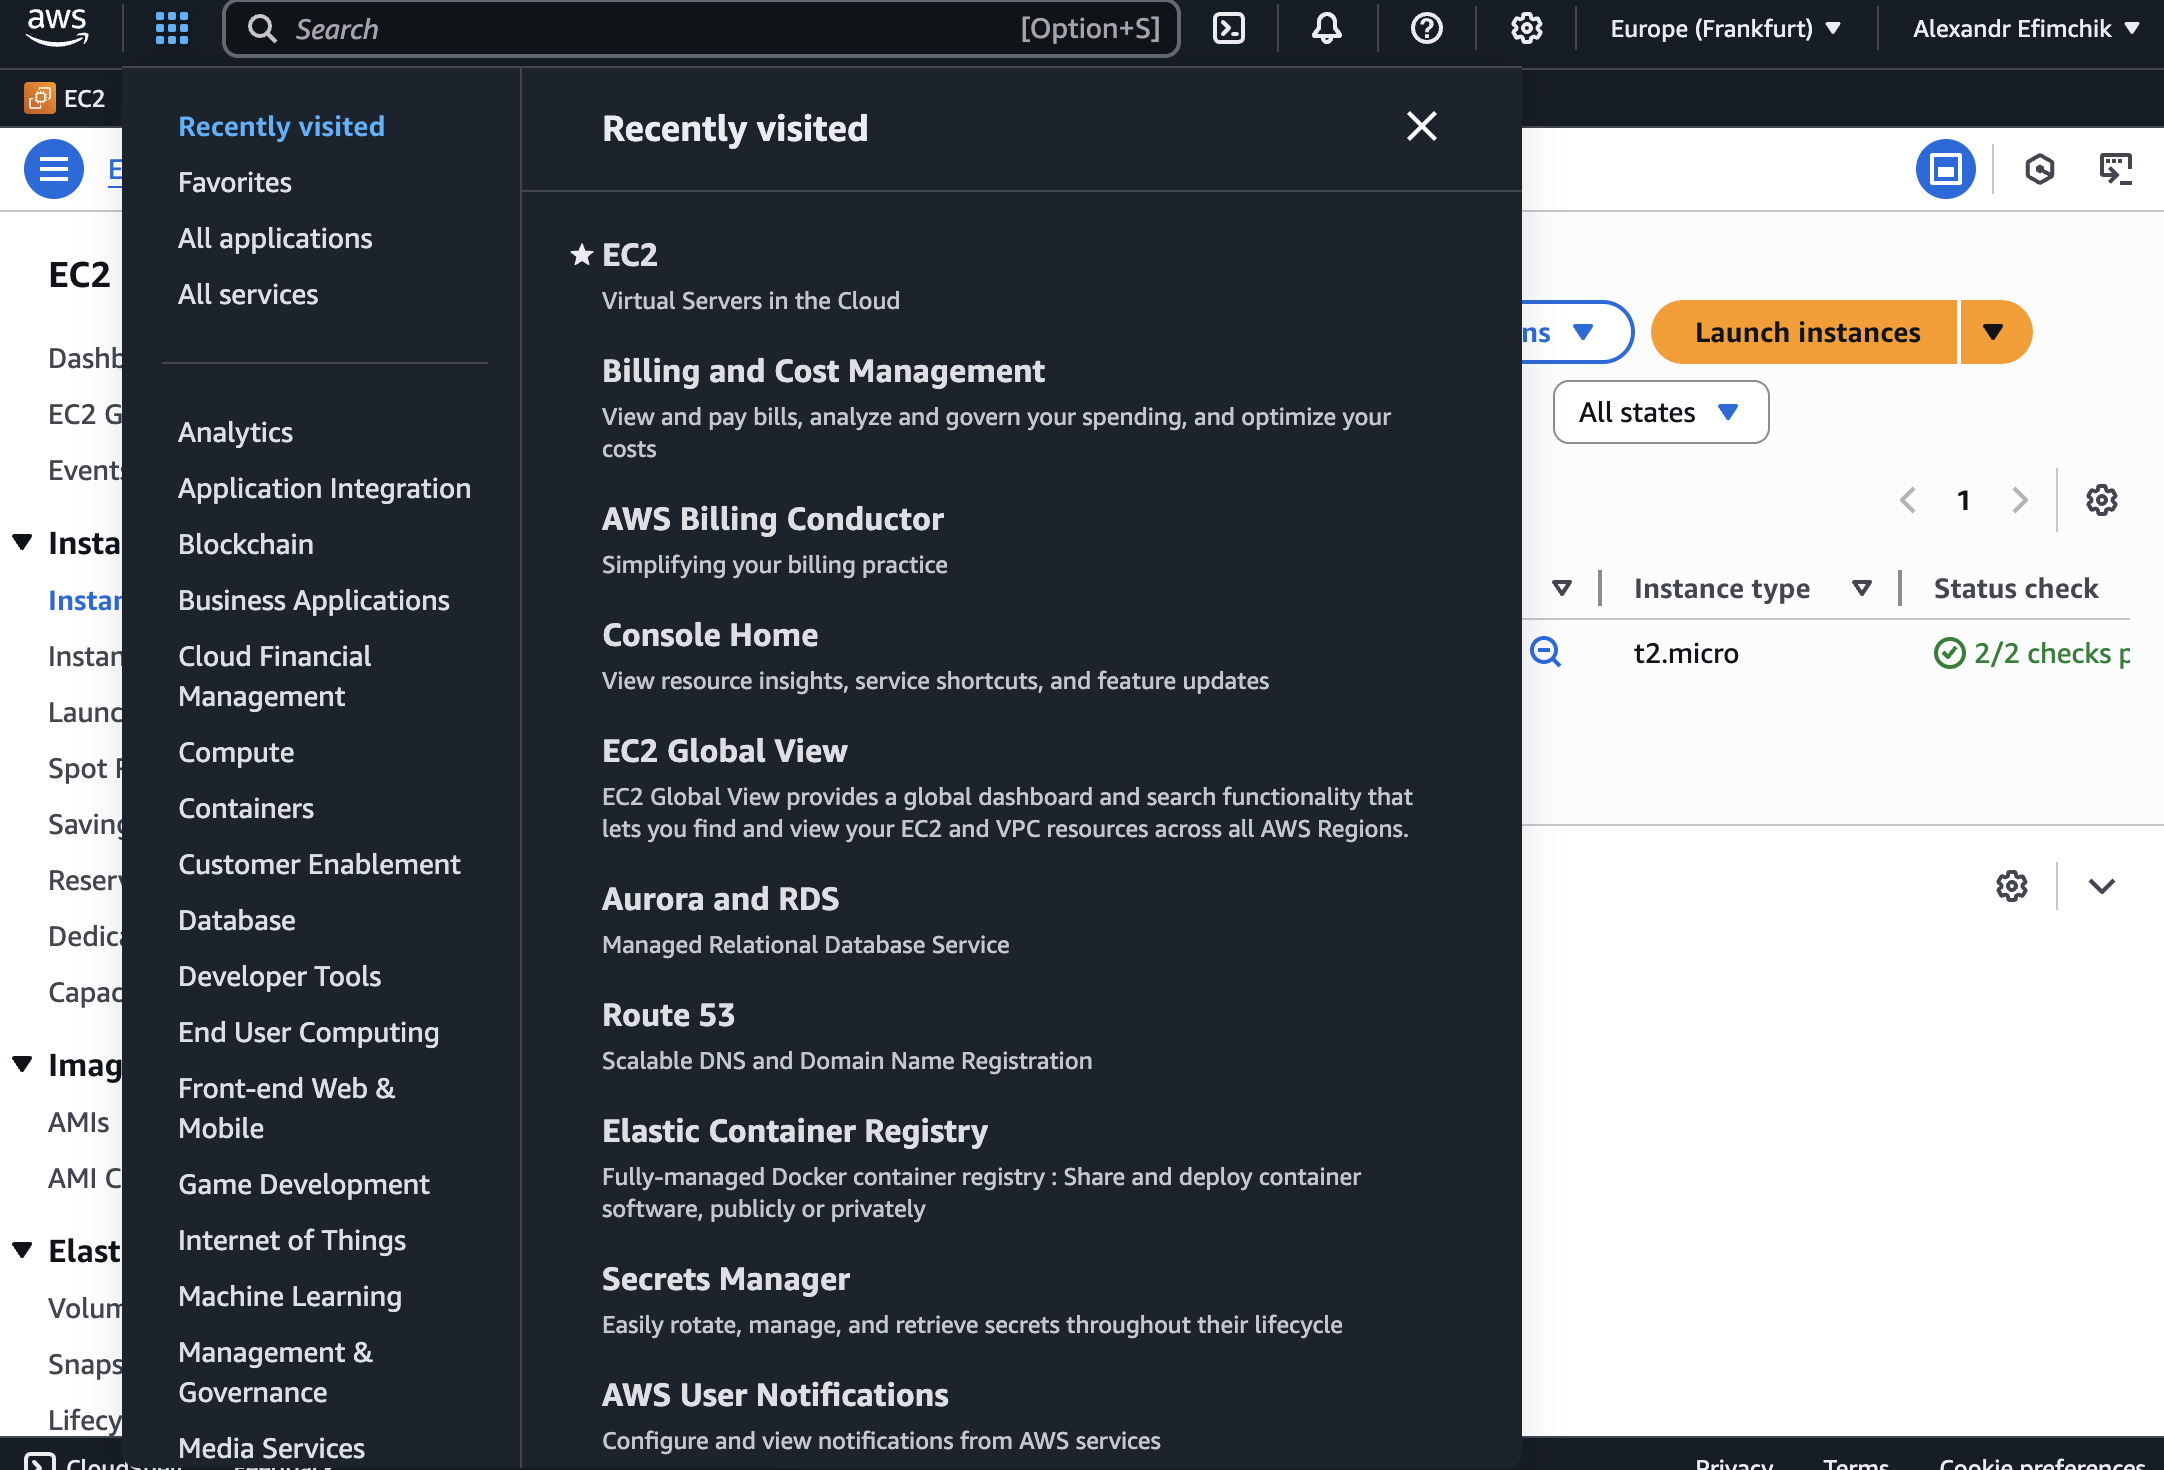
\includegraphics[width=0.7\linewidth]{\commonSecPathPrefix/../img/aws_admin.png}
    \caption{Интерфейс административной панели \textit{AWS}}
    \label{fig:user_guide:aws_admin}
\end{figure}

\subsubsection{Основные сервисы \textit{AWS}.} Среди таких сервисов можно выделить следующие:
\begin{enumerate}
    \item \textit{EC2 (Elastic Compute Cloud)} -- сервис для запуска виртуальных машин, предоставляющий масштабируемые вычислительные ресурсы.
    \item \textit{S3 (Simple Storage Service)} -- объектное хранилище данных для хранения файлов и резервных копий.
    \item \textit{RDS (Relational Database Service)} -- сервис для управления реляционными базами данных.
    \item \textit{EKS (Elastic Kubernetes Service)} -- сервис для управления \textit{Kubernetes}-кластерами, позволяющий развертывать и управлять контейнеризированными приложениями.
    \item \textit{IAM (Identity and Access Management)} -- сервис для управления пользователями и их доступом к ресурсам \textit{AWS}.
\end{enumerate}

\subsubsection{Применение \textit{AWS}.}
\textit{AWS} используется для создания и управления масштабируемыми и высокодоступными приложениями, поддерживает \textit{DevOps}-процессы и автоматизацию инфраструктуры. Он является одним из самых популярных облачных провайдеров для крупных организаций и стартапов, предоставляя гибкие решения для различных бизнес-задач.

\subsubsection{\textit{Yandex.Cloud}.}
\label{sec:yandex_cloud}
Платформа \textit{Yandex.Cloud} -- это облачная платформа от российской компании \textit{Yandex}, которая предоставляет широкий набор сервисов для разработки, развертывания и управления приложениями и инфраструктурой в облаке.
Среди доступных решений -- виртуальные машины, управляемые базы данных, контейнерные сервисы, хранилища, инструменты для обеспечения безопасности и мониторинга.
Платформа поддерживает как ручное управление ресурсами, так и автоматизацию с помощью \textit{API}, \textit{SDK} и инфраструктуры как кода \textit{(IaC)}. Панель администратора представлена на рисунке \ref{fig:user_guide:yc_admin}.

\begin{figure}[ht]
    \centering
    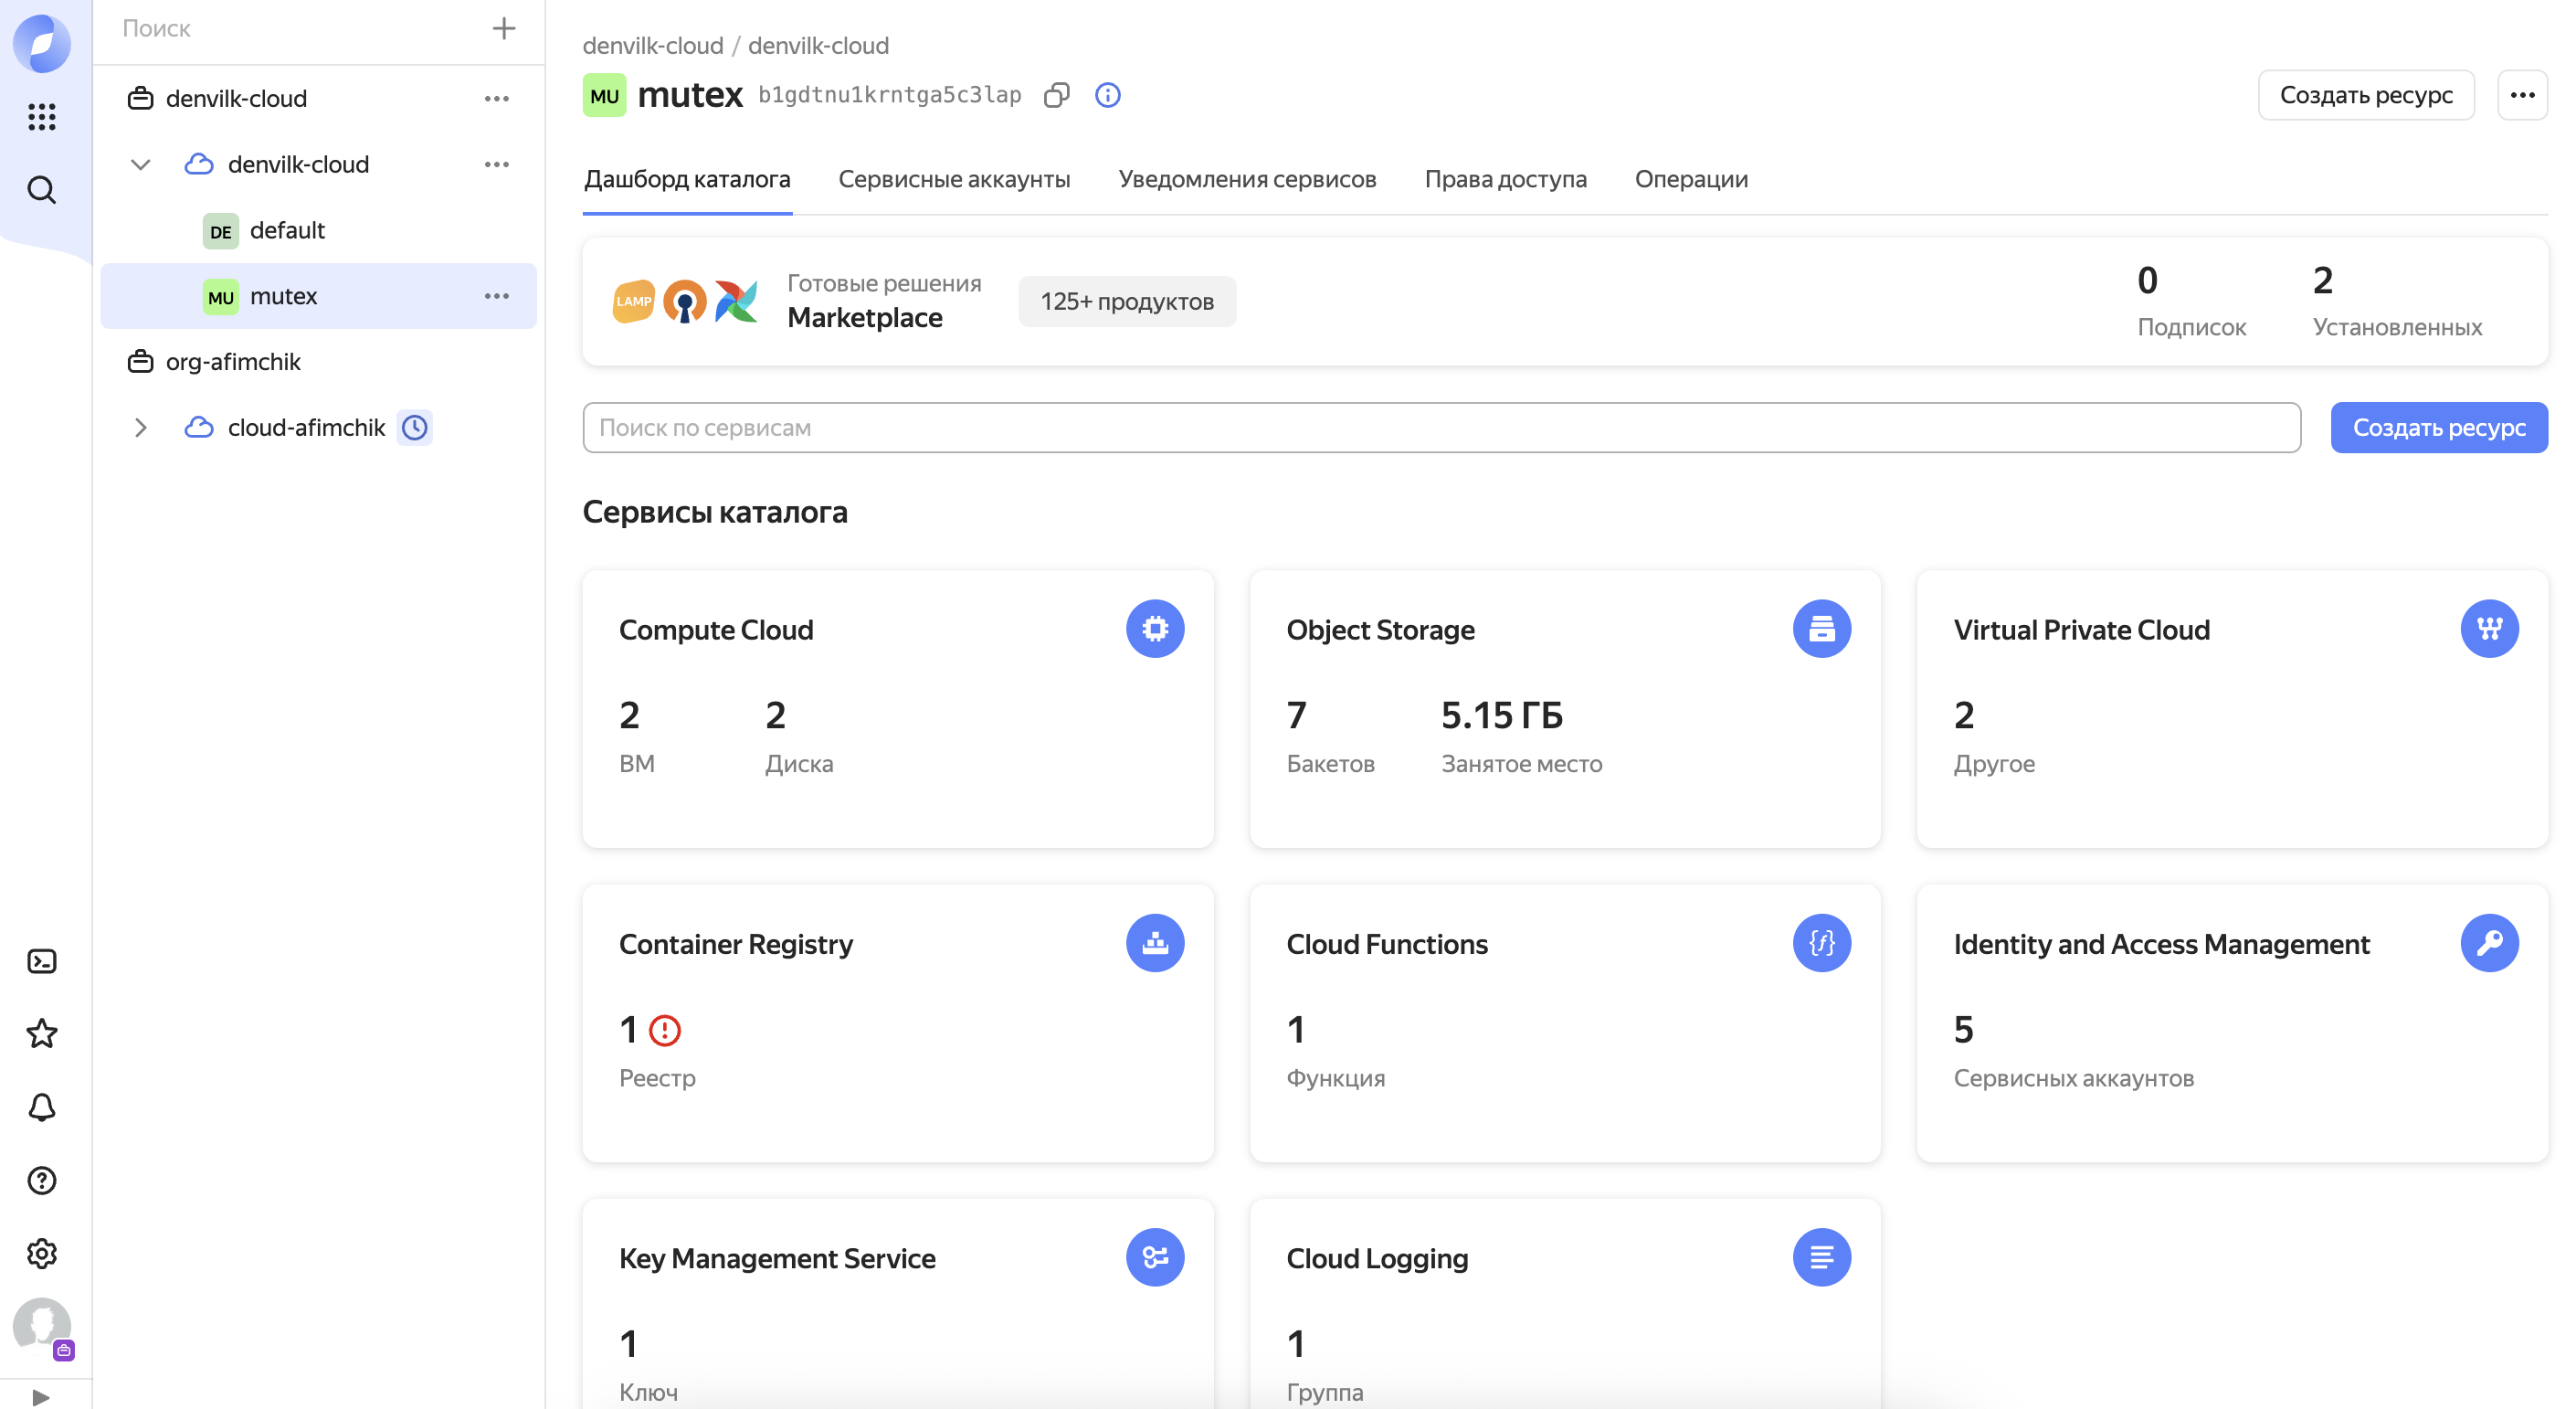
\includegraphics[width=0.7\linewidth]{\commonSecPathPrefix/../img/yc_admin.png}
    \caption{Интерфейс административной панели \textit{Yandex.Cloud}}
    \label{fig:user_guide:yc_admin}
\end{figure}

\subsubsection{Основные сервисы \textit{Yandex.Cloud}.} Среди таких сервисов можно выделить следующий ряд ключевых продуктов:
\begin{enumerate}
    \item \textit{Compute Cloud} -- сервис для запуска виртуальных машин с возможностью масштабирования ресурсов.
    \item \textit{Managed Kubernetes} -- управляемый сервис для развертывания и управления \textit{Kubernetes}-кластерами.
    \item \textit{Object Storage} -- объектное хранилище для хранения данных, резервных копий и медиафайлов.
    \item \textit{Yandex.DB} -- сервис для работы с реляционными и \textit{NoSQL} базами данных.
    \item \textit{Identity and Access Management (IAM)} -- система управления доступом пользователей и сервисов в облаке.
\end{enumerate}

\subsubsection{Применение \textit{Yandex.Cloud}.}
Провайдер услуг активно используется компаниями, ориентированными на российский рынок и требующими соблюдения местных стандартов безопасности и законодательных требований. Платформа поддерживает все необходимые инструменты для разработки, развертывания и масштабирования приложений в облаке, включая возможности для работы с \textit{Kubernetes} и виртуальными машинами.
